%!TEX root = ../main.tex

\documentclass[../main.tex]{subfiles} 
\begin{document}

\section{Simulation Study}\label{sec:simulation_study}
In the previous section I show how the model presented in this thesis can be useful in the identification of changes in skill prices in panel data. Following this identification strategy, changes in the prices of skills can be determined on the basis of the realized wages and task choices. In this section, I provide an exemplary application of this identification in the format of a simulation study\footnote{Program codes of this simulation study are openly available on GitHub: github.com/DaLueke/social\_skill\_prices}. 
\\
As part of this simulation study I, first, generate a representation of a panel data set that. The data generating process endogenously provides optimal task choices and according wages for each simulation period on the basis of potential task specific wages. In a second step, I rely on this simulated data in an estimation of skill prices following above described identification strategy.

\subsection{Data Generating Process} \label{sec:DGP}
% Generate 3 points in time so that I observe two intertemporal changes
%% Split into base period and a subsequent estimation period
% Generate potential wages
%% Skill prices: Exogeneously given. Constant in base period, changing in estimation period
%% Skill Endowments: Exogenous starting values, skill accumulation afterwards
%% Learning by doing process: Workers become better at the task they are doing relatively much.
% Penalty term: generate exogenous preferences for a task split
% Obtain optimally chosen task choice parameters by maximizing wages minus penalty
% Determine wage that results from optimal choice of tasks
% Can I find some nice way of visualizing my simulated data?
In order to produce a representation of a panel data set, the data generating process provides data on three points in time so that two inter temporal changes can be calculated. The first thereof serves as base period and the second as estimation period. Following the discussion of the model in section \ref{sec:implications-with-j=2}, this simulation is based on two different tasks. With the goal of simulating a utility maximization process in mind, both wages and penalty term need to be simulated (see equation \ref{eq:utility}). Therefore, I first describe the data generating process for potential task specific wages. Second, I present the parameterization of the penalty term.
\\
The wage function depends on task specific potential wages, which are assumed to result as sum of respective skill prices and individual skill endowments (see section \ref{sec:identifying-changes-in-skill-prices}, particularly equation (\ref{eq:potential_wages})). Prices of each skill in each period are exogenous in the model. In this simulation study specifically, they are modeled to be constant during the base period and changing during the estimation period. In order to facilitate the evaluation of estimation results, the data generating process used in this simulation study is specified to have a deterministic change in relative prices.
\\
Skill endowments at the first observed point in time are randomly drawn from a normal distribution. In subsequent periods, skills endowments experience an accumulation that is modeled as a learning by doing process. In particular, workers gain relative skill in that task, which they execute to a relatively large extent. The stronger a worker focuses on one single task, the larger is the gain in relative skill herein. This results in a skill accumulation that depends on task choices, hence can be estimated using these task choices. It therefore meets the conditions for being estimated using the method described in section \ref{sec:model_estimation}.
\\
In accordance to the normalization of potential wages introduced in section \ref{sec:implications-with-j=2}, potential wages of task one are normalized to zero so that potential wages of task two need to be understood as relative sizes. Specifically, a skill endowment for task two that is positive indicates that a worker has a comparative advantage in doing this task and vice versa for negative skill endowments. Analogously, a relative skill price that is larger than zero implies a higher compensation for executing task two.
\\
The penalty term is a function of individual time allocation preference, captured in parameter $b_i$. For this simulation study this parameter is generally assumed to be uniformly distributed within some borders $\{b_{low}, b_{high}\}$ with $b_{low}, b_{high} \in [0, 1] \; \text{and} \; b_{low} \leq b_{high}$. The resulting interval is centered at the equal split of work time on both tasks, so that neither task is systematically preferred to the other. Additionally, it is assumed that workers dislike strong specialization (section \ref{sec:utility-max-problem}). To do justice to this assumption, the limits of the parameter for preferred allocations should, therefore, not be chosen in the extremes. In the data generated process that is used for the simulation study, the borders of individual time allocation preferences are set to $b_{low} = 0.3$ and $b_{high} = 0.7$.
\\
For this simulation study, I use a quadratic specification of the penalty function, i.e. the penalty exponent is set to $\phi = 2$. This specification meets  the assumed properties of the penalty function. 
% TODO: Add plot with optimal task choices to show that these are (1) not in the extremes and contain no corner solutions. (2) they are centered in the middle of the distribution, accounting for the slightly higher prices in task 2 of course, so slightly skewed dist towards task 2. 
At the same time, it results optimal task choices that are a linear function in relative potential wages, which makes the linear interpolation of inter temporal changes in task choices an exact solution. The penalty weight parameter $\tau$ is set to a value of $\tau = 15$ in this data generating process. This weight is chosen so that neither realized wages nor the penalty dominates the utility function.
% TODO: Add graph with sizes of both parts as proof of this statement.
While the first case could result in a large number of corner solutions where every worker focuses on the task with higher potential wage, the second case would produce a dataset in which workers mostly stick with their preferred task choice so that potential wages, and more importantly changes thereof, impact task choice very little.
\\
Based on both, potential wages and the penalty term, the optimal task choice parameter $\lambda_{i,t}^*$ can be obtained in each period by maximizing the individual utility (i.e., realized wage lessened by the penalty term). Furthermore, resulting realized wages can be calculated using this optimal task choice. Utilizing both, task choices and resulting wages, allows to estimate the change in relative skill prices on which the data generating process is based. In the next section, I show how changes in skill prices can be estimated relying on the identification strategy discussed in section \ref{sec:model_estimation} and using data generated by the process described in this section.
\\
A representation of the simulated data can be seen in figure \ref{fig:simulated_data}. Particularly, the figure shows the combinations of optimal task choices $\lambda_{i,t=0}^*$ and realized wages $w_{i,t=0}$ for all $N=100$ simulated workers in one of the Monte Carlo iterations. From the graphic it can be seen that task choices (horizontal axis) are distributed around the equal split, with no worker engaging in an extreme focus on either one of the tasks. The histogram of realized relative wages (vertical axis) shows an increased frequency at the center of the distribution around a relative wage of zero. Both, relatively high and low realized relative wages are less frequent.
\\
In the data generating process, the relative skill price of task two is fixed at $0.05$ which implies that the skill price of task two is $5 \%$ higher than the price of task one. This setting should result positive relative realized wages for workers that spend the majority of their working time on task two. Indeed, workers who have higher $\lambda_{i,t}^*$ tend to earn relatively high wages. This impression is supported by the position of a regression line through the point cloud (black dotted line in figure \ref{fig:simulated_data}).

\begin{figure}[!htbp]
	\centering
	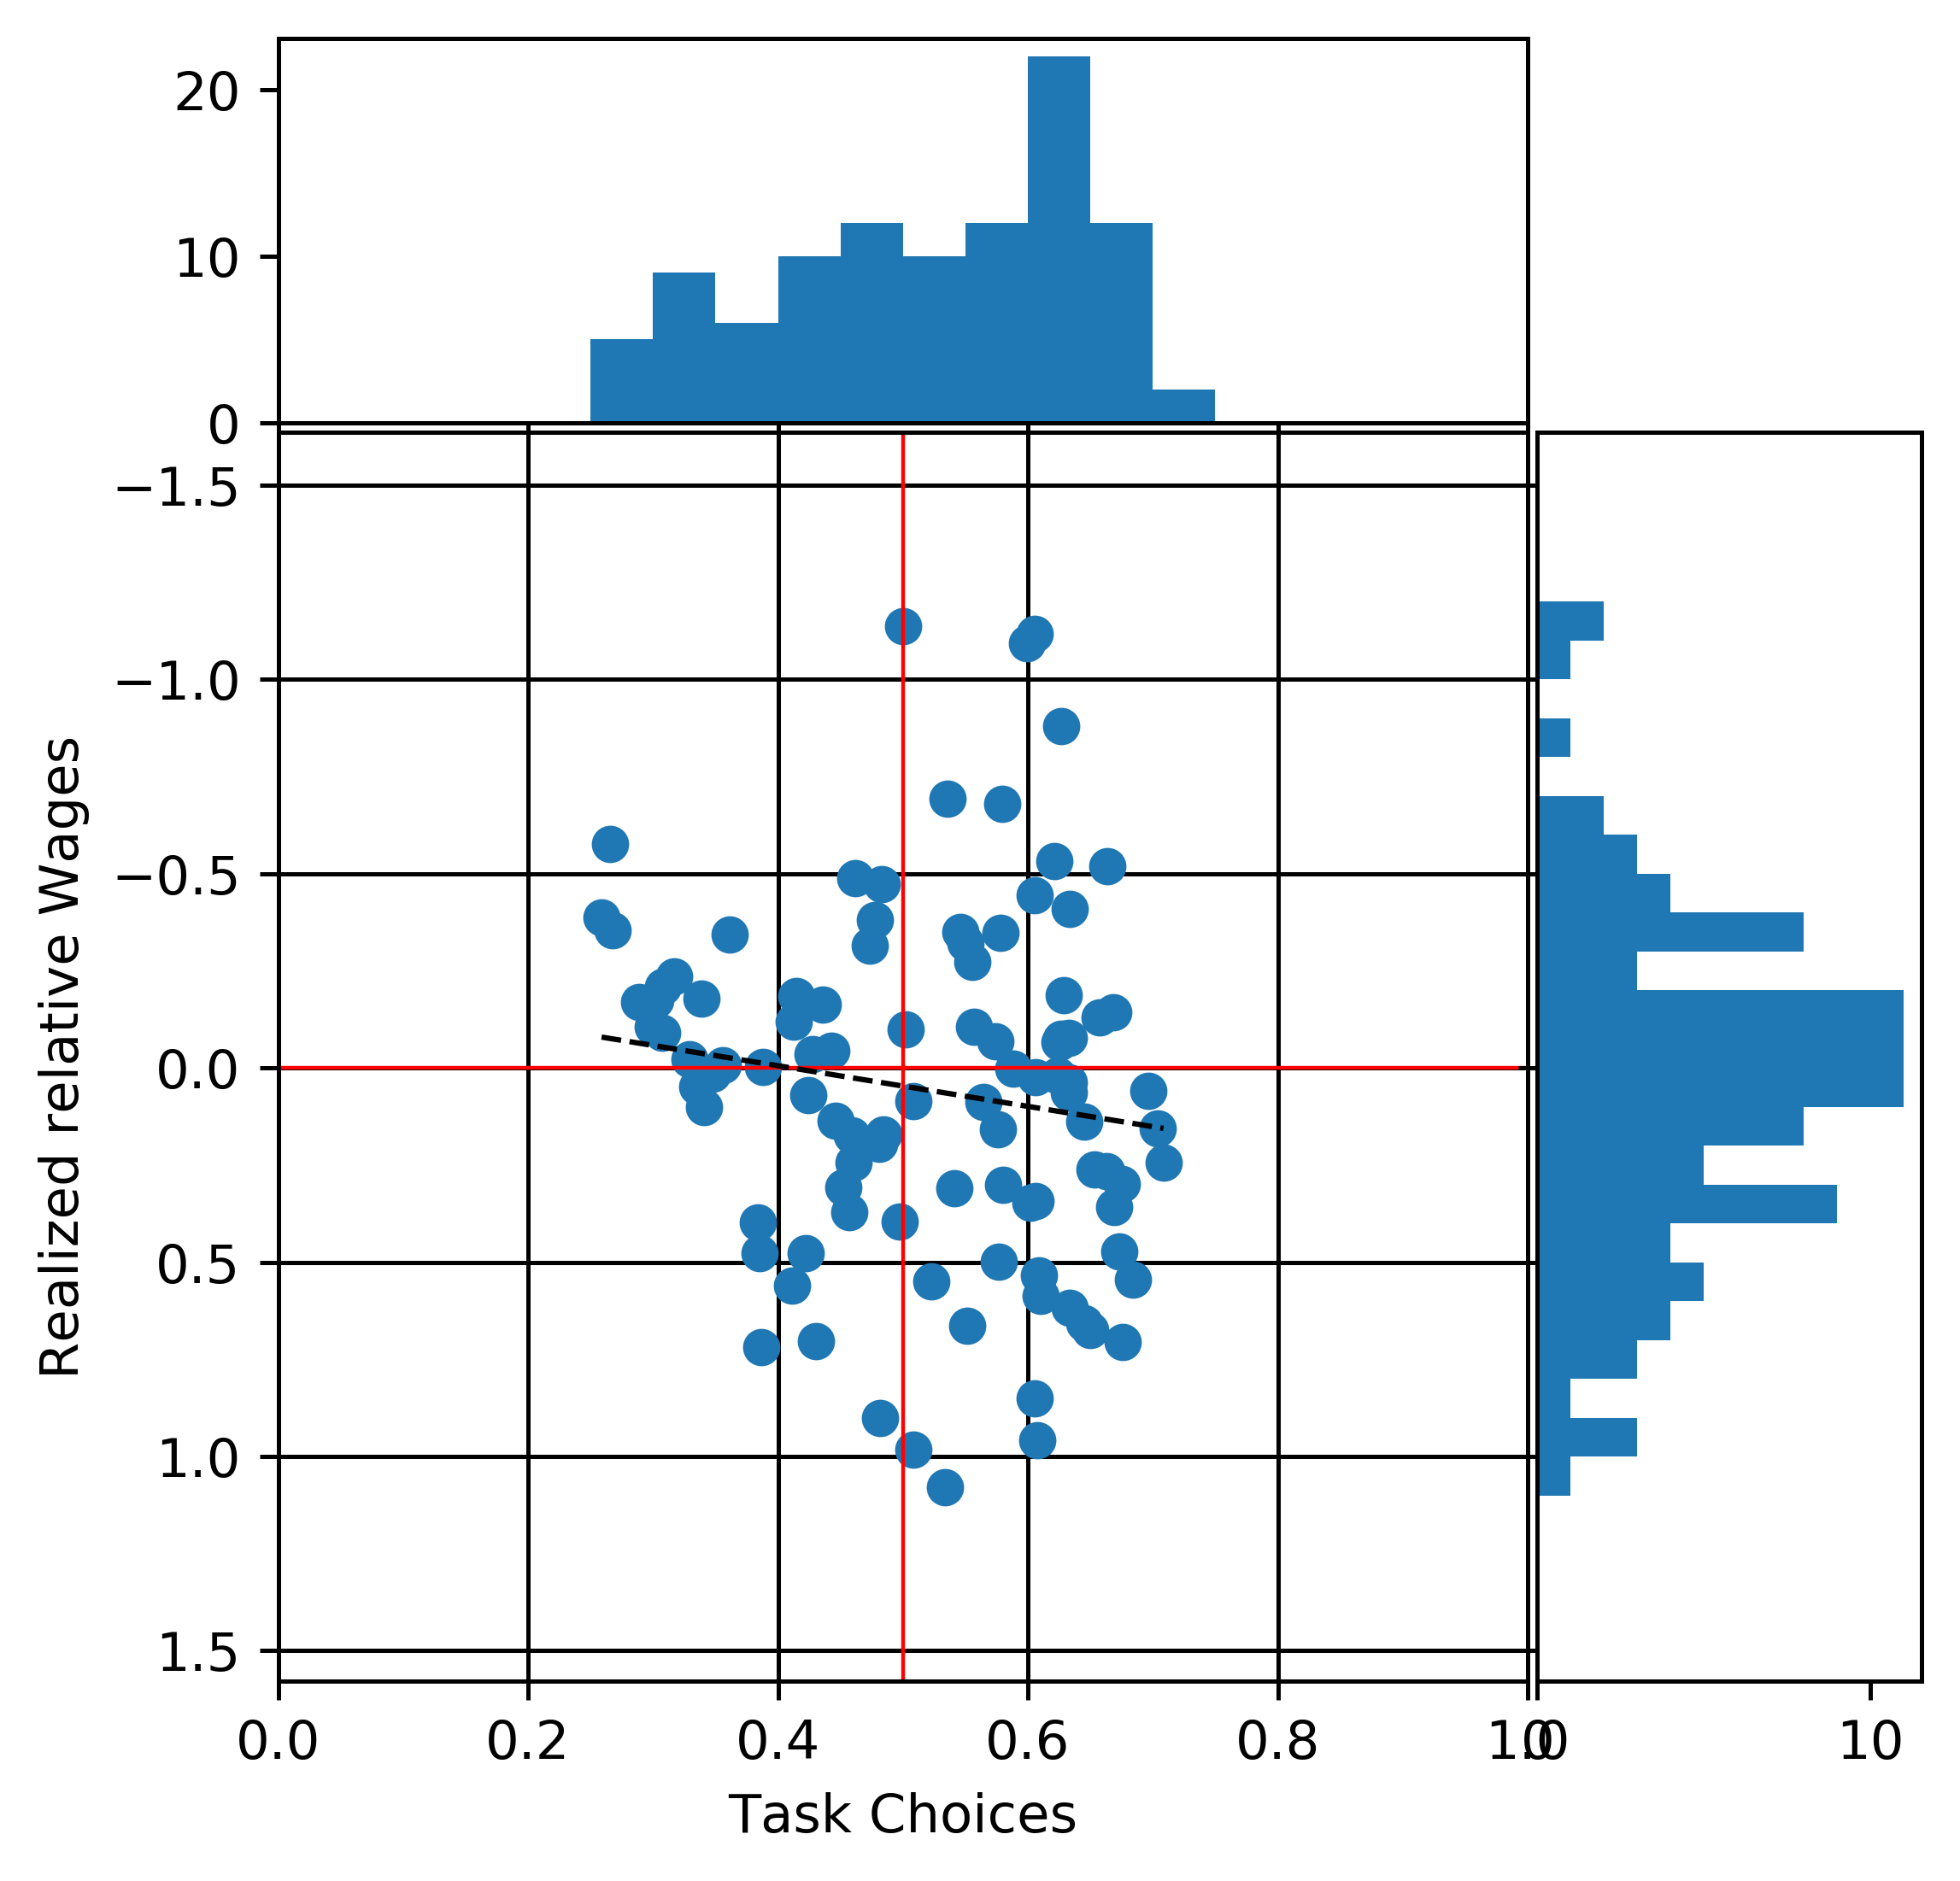
\includegraphics[scale=0.7]{./FIG/simulated_data.png} 
	\caption{Simulated data resulting from a data generating process that is specified as described in section \ref{sec:DGP}. This figure illustrates $N=100$ combinations of realized wages and optimal task choices in a scatter plot with histograms of the respective variables along each axis. The dashed line results from an OLS fit.}
	\label{fig:simulated_data}
\end{figure}

\FloatBarrier
\subsection{Monte Carlo Estimation of Skill Prices} \label{sec:MC_estimation}
% Following the identification strategy presented in section 2.4.:
%% use base period (without price changes) to estimate effects of changes in skill endowments as well as pentalty term 
%%% Present regression table: Show that I need to drop some regressors (multicol.), show that I capture most of the variance, show that estiates are highly significant.
%% use these estimations to calculate a "residual wage change" in estimation period, i.e., adjust wage changes for above mentioned effect
%% Regress residual wage change on mean lambda
%%% Show regression rslt: high significance, point estimate, R^2 should be relatively high in this model, too
% Present results from MC-Simulation (distribution of point estimates)
% Find reasons for bias in estimation: Why is my estimate too high? 
%% Do I not completely capture skill changes (same regressor)? 
%% Does dropping regressors in first step result in inappropriate estimators and, thus, biased estimations?
% overall: Model allows to obtain a close estimate of true price changes
%% Potentil problems and (1) Why they are not that relevant in real data and (2) what can be done to mitigate 
This section presents the results of a Monte Carlo estimation of changes in skill prices and serves as a proof of concept of the model I present in section \ref{sec:tractable-model-of-cont-task-choice} of this thesis, particularly of the estimation strategy discussed in section \ref{sec:model_estimation}. For this purpose it relies on data generated in the process described in previous section.
\\
The estimation of skill prices consists of three steps: First, I make use of a base period to estimate the effects of skill accumulation and changes in the penalty term in the absence of changes in skill prices. Second, observed wage changes of a subsequent period are adjusted for these previously estimated effects. Third, I estimate changes in skill prices based on these residual wage changes. Each of these steps is repeated $M=1000$ times in a Monte Carlo estimation, each time considering data on $N=100$ simulated individuals.
\\
In the particular model discussed in this work both, changes in skills and changes in the penalty term from $t-1$ to $t$, are functions of task choices $\lambda_{i,t-1}^*$ and $\lambda_{i,t}^*$. This can be seen from equation (\ref{eq:wage_change}). Specifically, skill accumulation results as a function of the mean task choice of both periods, $\bar{\lambda}_{i,t}^*$. The change in penalty term, however, results as a polynomial of degree $\phi$ of these optimal task choices (see appendix \ref{app:derive_changes_penalty_term} for a derivation of this result). In the particular setting of the data generating process that is used in this simulation study, it is assumed that $\phi = 2$. In this case, changes in the penalty term can be shown to be equivalent to the expression in equation (\ref{eq:changes_in_penalty}) below as shown in appendix \ref{app:derive_changes_penalty_term}. Therefore, both $\lambda_{i,t-1}^*$ and $\lambda_{i,t}^*$ as well as their squared values need to be included to capture changes in skill endowments and penalty terms.
\begin{equation}\label{eq:changes_in_penalty}
	\Phi_{i}(\lambda_{i,t}^*) - \Phi_{i}(\lambda_{i,t-1}^*) = \lambda_{i,t-1}^{*2} + \lambda_{i,t}^{*2} + 2b_i(\lambda_{i,t-1}^* + \lambda_{i,t}^*) 
\end{equation}
% Now find the model that is actually used in estimation
% Due to strong correlation of lmbs, I suspect i will have to drop some. So go check different specifications and see how they perform in 
% (a) modelling base period and 
% (b) adjusting in estimation period
In an estimation of skill accumulation and changes in the penalty term, however, not all of these regressors can be included due to their strong multicollinearity. Not only will each task choice be correlated with its square. In addition, task choices of subsequent periods will be correlated. This is for two reasons: First, optimal task choices (equation (\ref{eq:lmb_opt})) are a function of potential wages. Potential wages, in term, are modeled as the sum of log skills and log skill prices. By the assumption of skill accumulation as a learning by doing process, potential wages will correlate between periods and, thereby, optimal task choices will be correlated as well. Second, optimal task choices are a function of the allocation preferences $b_i$ which are modeled to be time-invariant. As seen from figure \ref{fig:corr_heatmap}, all task choice related regressors are, indeed, almost perfectly correlated.
\\
\begin{figure}[!htbp]
	\centering
	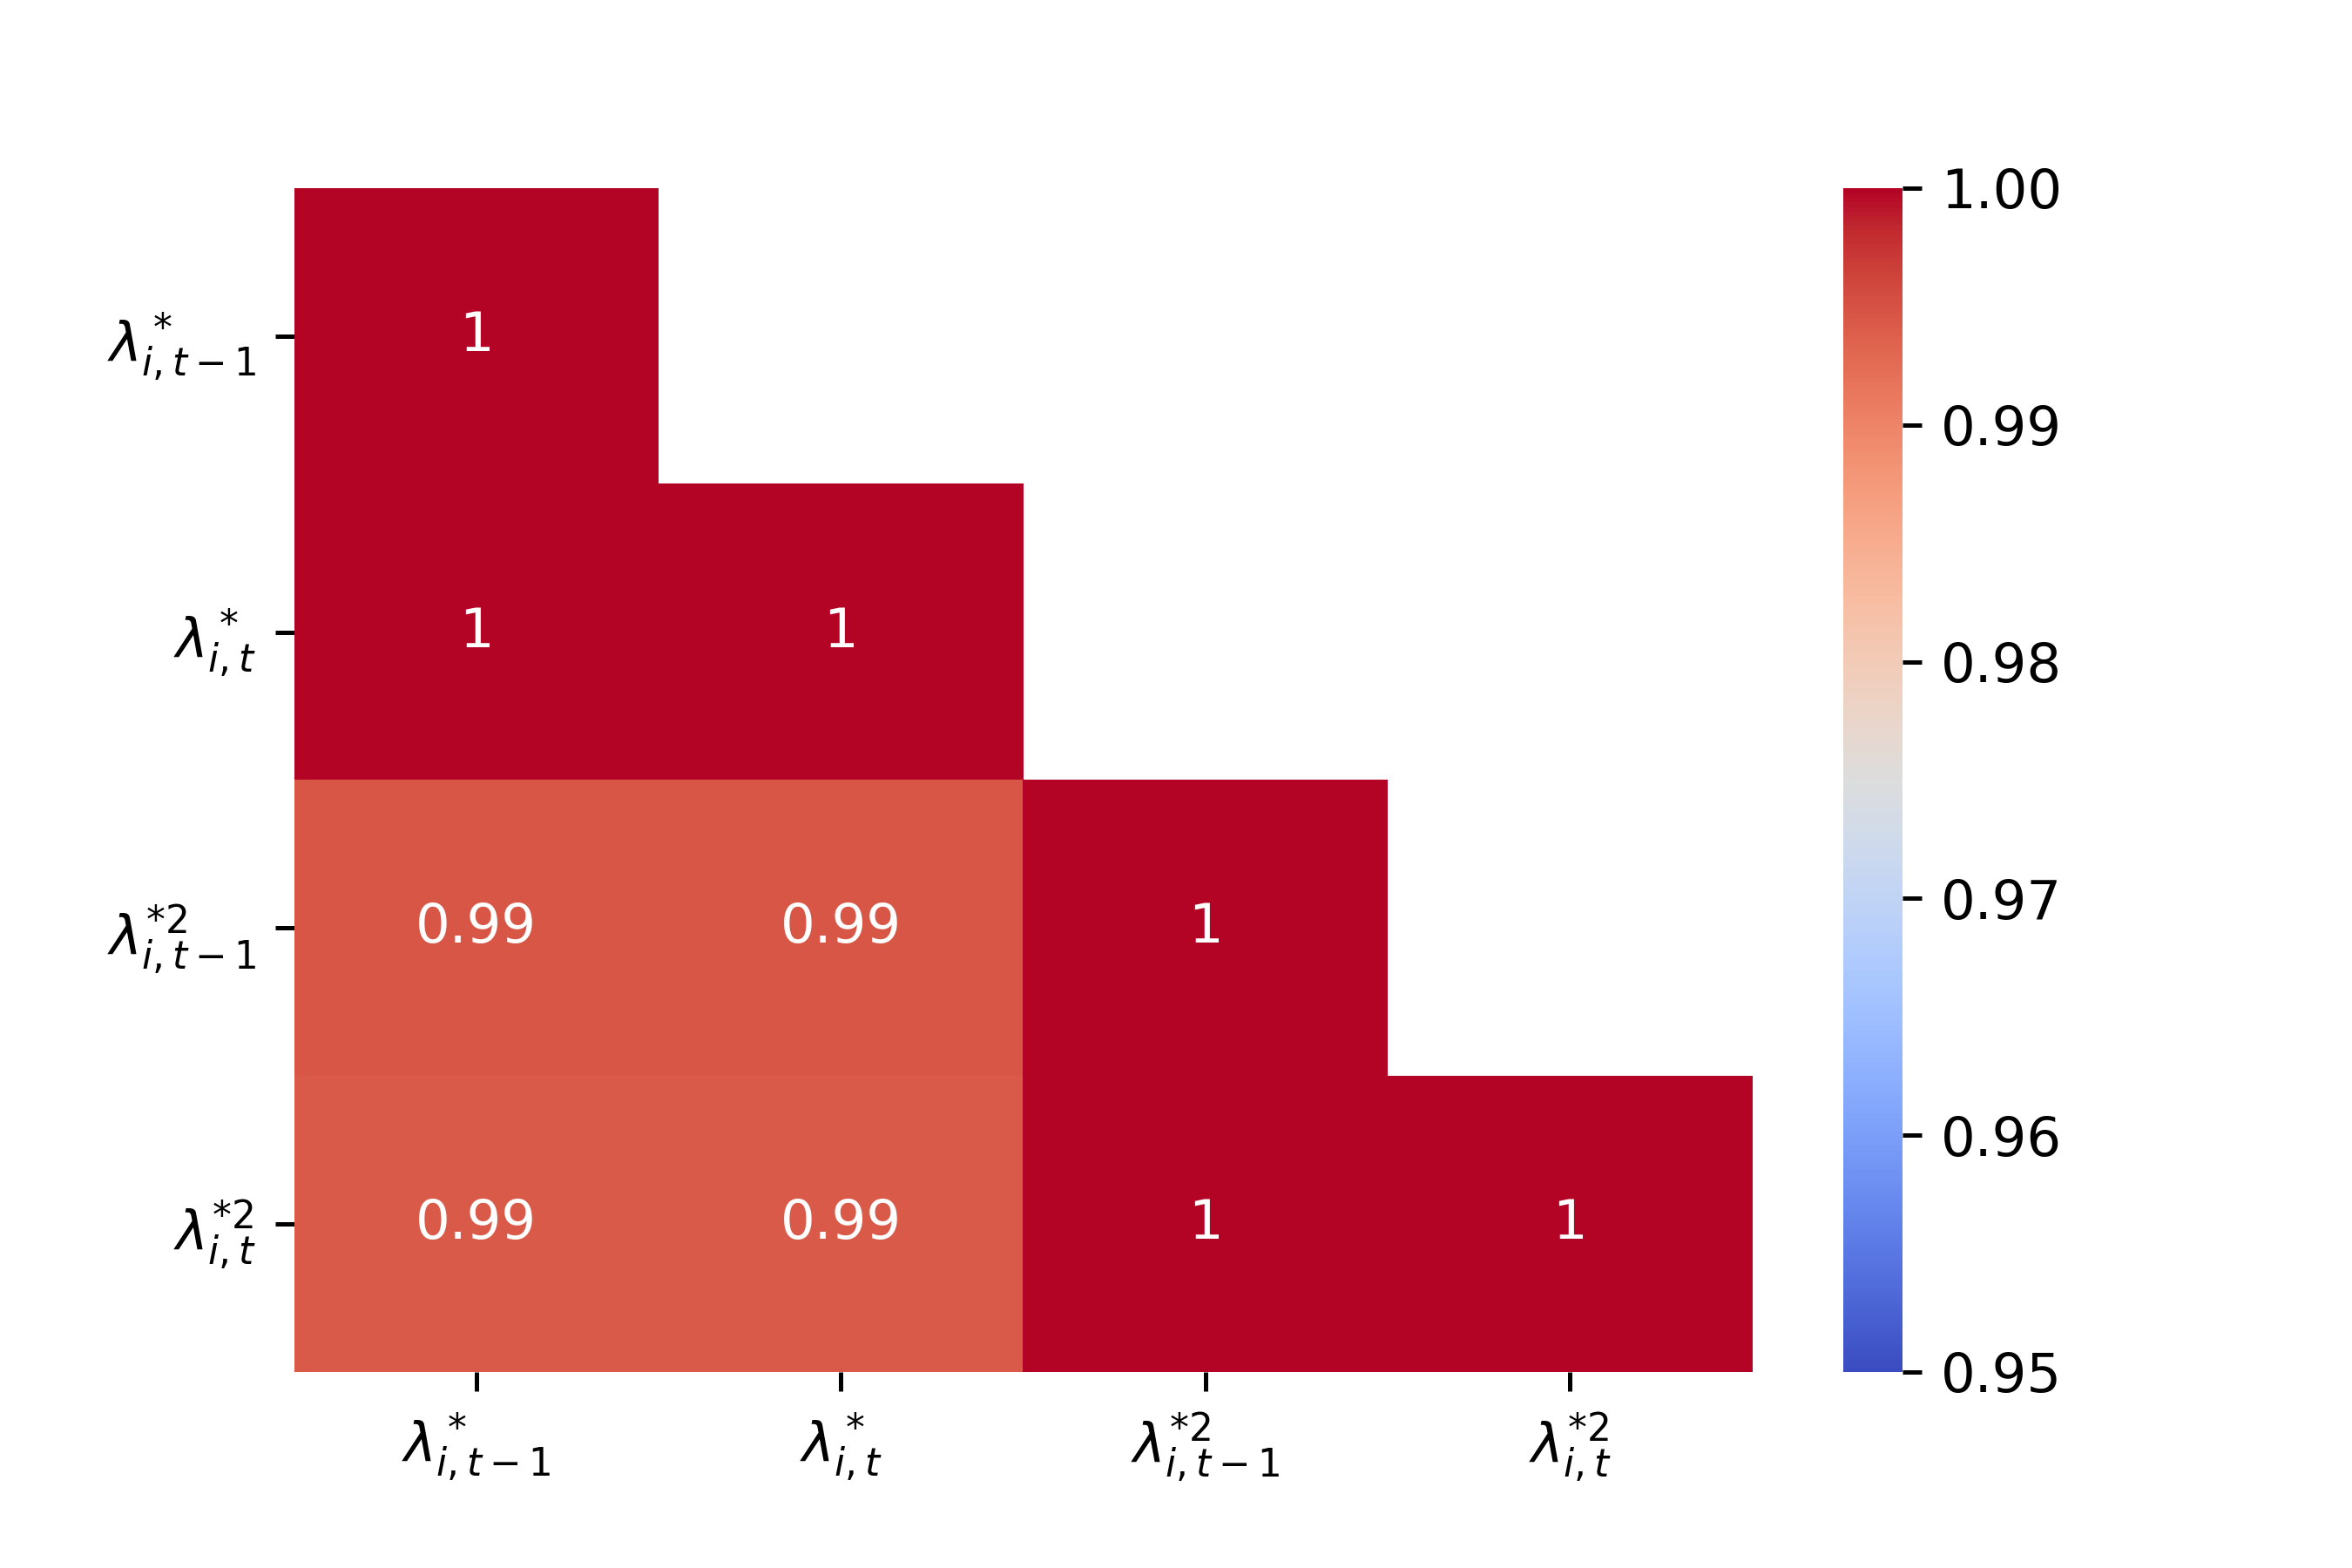
\includegraphics[scale=0.75]{./FIG/corr_heatmap.png} 
	\caption{Heatmap of correlation coefficients of task choices in periods $t-1$ and $t$ of the base period as well as their squared values. It should be noted that the scale is compressed and only covers values between 0.95 and 1.0 to make the small differences visible.}
	\label{fig:corr_heatmap}
\end{figure}
In order to address potential multicollinearity, only task choices of the later period are included as regressors. 
% TODO: Show that alternative specification (i.e. only of earlier period) does not change results a lot. Argue why it does change it a little. 
As seen from the estimation result in table \ref{tab:base_period_regression_rlst}, this estimation specification appears to fit the simulation data well with an adjusted $R^2$ of 0.997. Each iteration of the Monte Carlo estimation is based on $N=100$ simulated observations. While this number is small enough to keep the computational load low, the resulting estimates have small standard deviations and high significance ($p<0.001$ for both estimates).
\\
\begin{table}
\begin{center}
\begin{tabular}{lclc}
\toprule
\textbf{Dep. Variable:}    & adj. wage change & \textbf{  R-squared (uncentered):}      &     0.997   \\
\textbf{No. Observations:} &       100        & \textbf{  Adj. R-squared (uncentered):} &     0.997   \\
\textbf{F-statistic:}      &  1.721e+04       & \textbf{  Prob (F-statistic):}          & 1.62e-125   \\
\bottomrule
\end{tabular}
\begin{tabular}{lcccccc}
                  & \textbf{coef} & \textbf{std err} & \textbf{t} & \textbf{P$> |$t$|$} & \textbf{[0.025} & \textbf{0.975]}  \\
\midrule
\textbf{$\lambda_{i, t}^{*}$}   &      -0.4803  &        0.004     &  -128.958  &         0.000        &       -0.488    &       -0.473     \\
\textbf{$\lambda_{i, t}^{*2}$} &       0.9633  &        0.006     &   150.591  &         0.000        &        0.951    &        0.976     \\
\bottomrule
\end{tabular}

\end{center}
\caption{Results of an OLS estimation of wage changes in the base period on both, $\lambda_{i, t}^{*}$ and $\lambda_{i, t}^{*2}$. This estimation result is from one of the $M = 1000$ simulated datasets used in the Monte Carlo estimation. Regressors do not include a constant because the true model intersects the point of origin due to the normalization of $w_{i,j=1,t} = 0$.}
\label{tab:base_period_regression_rlst}
\end{table}
In each of the $M=1000$ iterations of this Monte Carlo estimation, changes in skills and penalty term are estimated using this regression model. After that, wage changes of the subsequent time period are adjusted for the product of the later period's task choices and the estimated coefficient of the base period. Resulting residual wage changes are the basis of the estimation of changes in skill prices.
\\
\begin{figure}[!htbp]
	\centering
	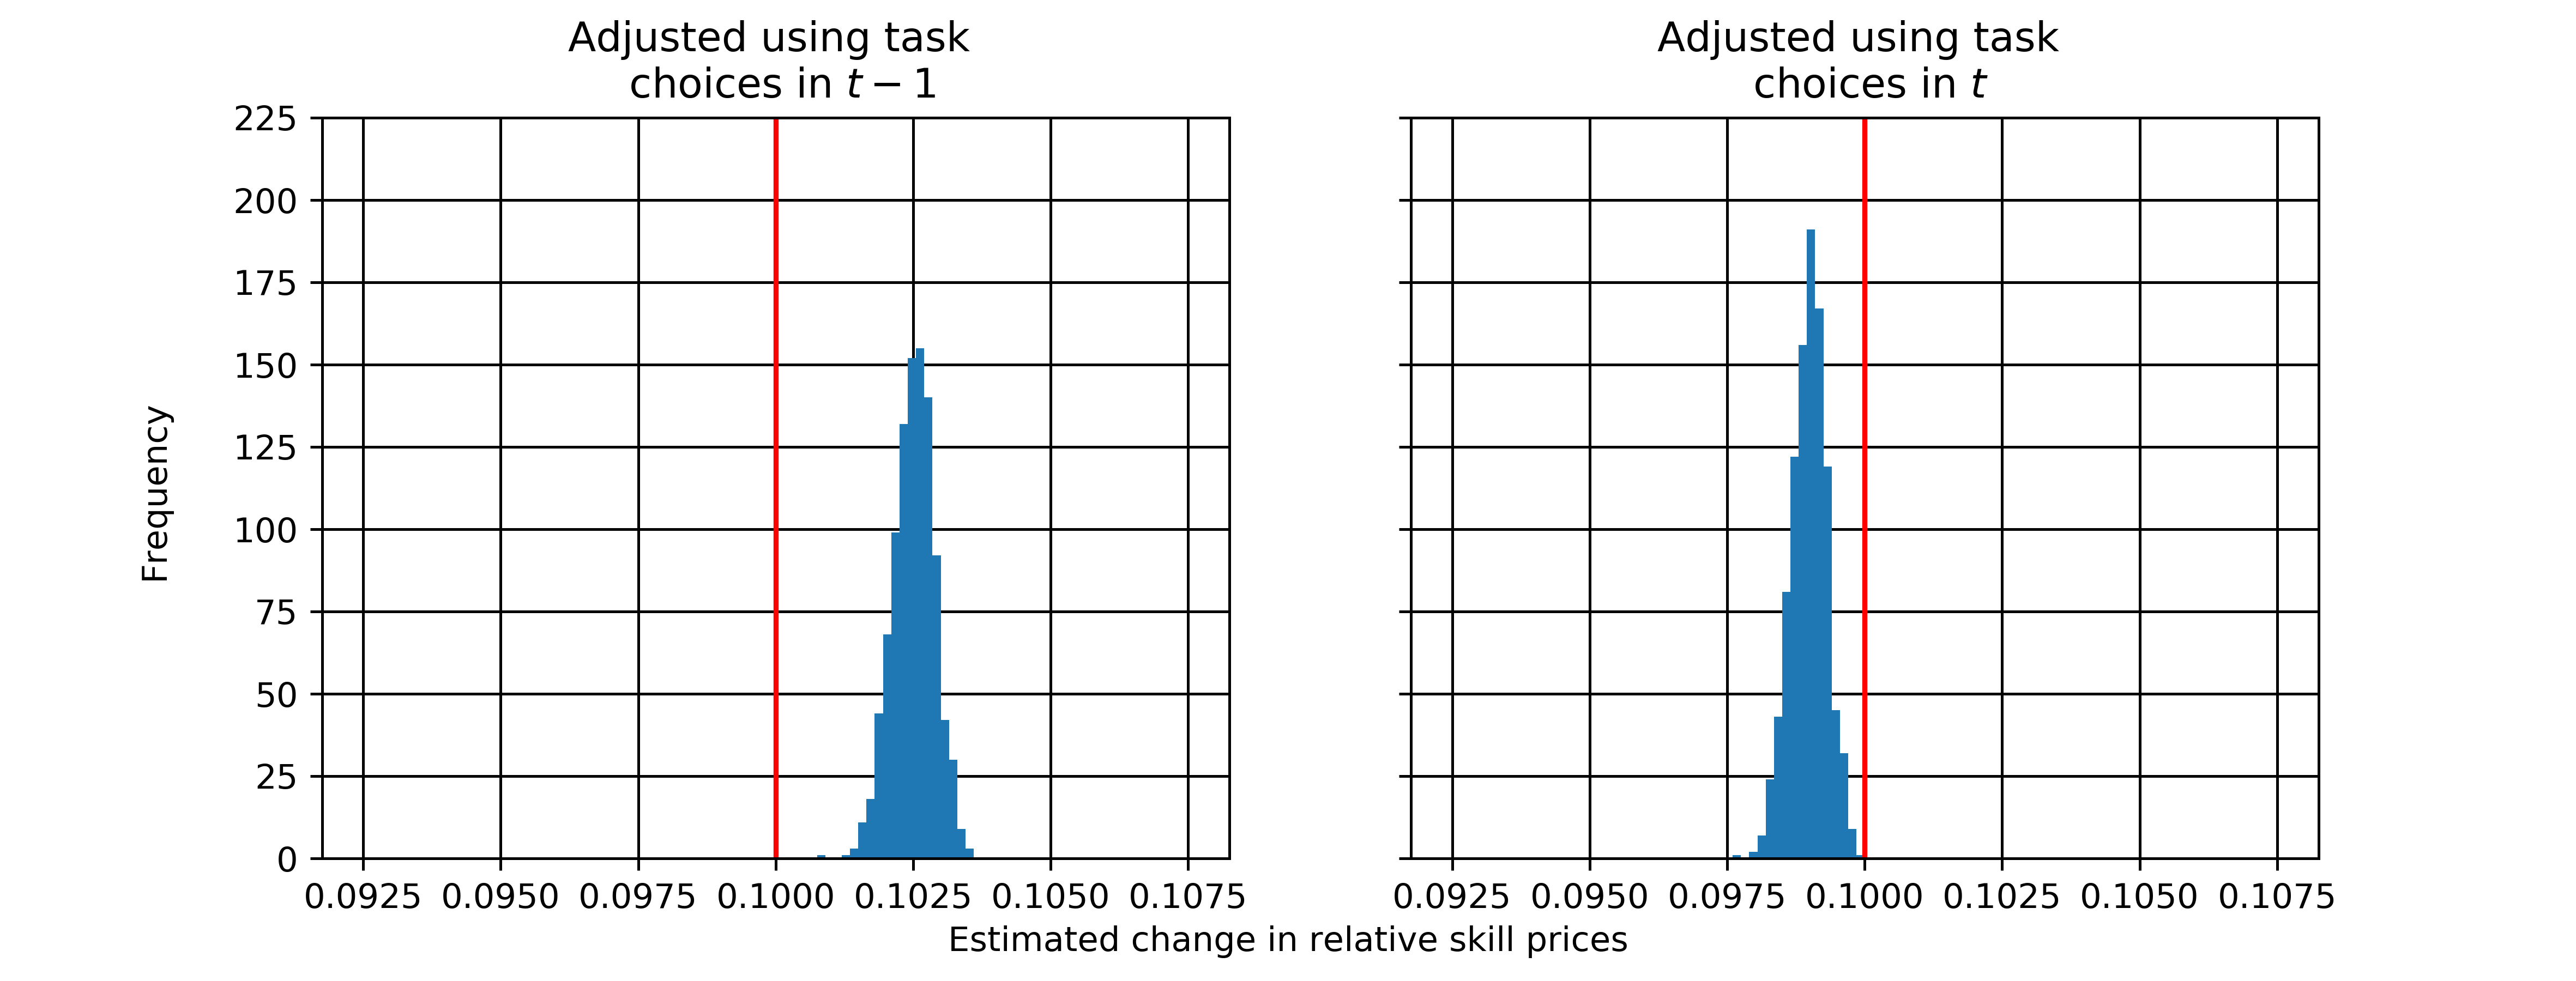
\includegraphics[scale=0.75]{../FIG/MC_estimation_rslt.png} 
	\caption{Histogram of the result of $M=1000$ Monte Carlo estimations of changes in relative skill prices. The true price changed used in the data generating process is $0.1$.}
	\label{fig:MC_est_rslt}
\end{figure}
Figure \ref{fig:MC_est_rslt} presents a histogram of the estimation results for $M=1000$ Monte Carlo estimation in a model with true changes in relative prices of $0.1$. While the peak of the distribution of estimation results is slightly below this true change in relative prices at approximately 0.0995, the true value of $0.1$ is well covered by this distribution.
\end{document}